\chapter{Drupal Structure}
\label{ch:drupal_structure}

\section{Core concept}
Drupal uses entities. The concept of entities is in reality a pretty complicated one, but mostly to developers. This is because Drupal’s API contains some nifty functionality concerning Entities, but to most webmasters, site builders and themers alike, Entities don’t have to be that complicated. 
Entities are like furniture, for example a bookshelf. By itself, a bookshelf doesn’t do very much. It’s actually not that interesting, it just IS. But add some books, change the shelving, mix it up a bit and add some pictures, and the bookshelf becomes a design centre piece of your living room.... Now imagine you could reuse those pictures in different sizes or frames... all over your living room! You could definitely throw together some interesting compositions! 
\subsection{Fields} 
All of the entities in Drupal are ‘fieldable’, meaning we can add fields to them. A field is a reusable piece of content. A field has a primitive data type like Boolean or Decimal or Text or Image or file etc. With the help of fields we define custom content types, taxonomies etc.... 

\subsubsection{Field Types} 
General: 
\begin{itemize}
    \item Boolean - On/off checkbox 
    \item Comments - This field adds a ‘Add comment’ form and the submitted comments 
    \item Date 
    \item E­mail 
    \item Link 
    \item Timestamp
\end{itemize}

Number: 
\begin{itemize}  
    \item List (float) ­ A list of numeric values. 
    \item List (integer) ­ A list of numeric values. 
    \item Number (decimal) 
    \item Number (float) 
    \item Number (integer) 
\end{itemize}

Reference: 
In Drupal we can link pieces of content to each other by using a reference field, referenced items can be partially or fully displayed if you want to. All the following entities can be referenced: 
\begin{itemize}  
    \item Content 
    \item File 
    \item Image 
    \item Taxonomy term 
    \item User 
    \item Other 
\end{itemize}

Text:
\begin{itemize}
    \item List (text) ­ A list of text values. 
    \item Text (formatted) ­ A single line text field, for short texts, allows formatted text (like html or wysiwyg). 
    \item Text (formatted, long) ­ A text area with multiple rows, allows formatted text (like html or wysiwyg). 
    \item Text (formatted, long, with summary) ­ Same as above but with an extra text area to add a summary. 
    \item Text (plain) ­ A single line text field, for plain unformatted text. 
    \item Text (plain, long) ­ A text area with multiple rows, for plain unformatted text. 
\end{itemize}


\section{Structural elements}
Drupal core defines eight types of structural elements. To see an overview of those elements click on the Structure button in the administrative menu (Figure \ref{fig:struct_elements}).

\begin{figure}[H]
    \centering
    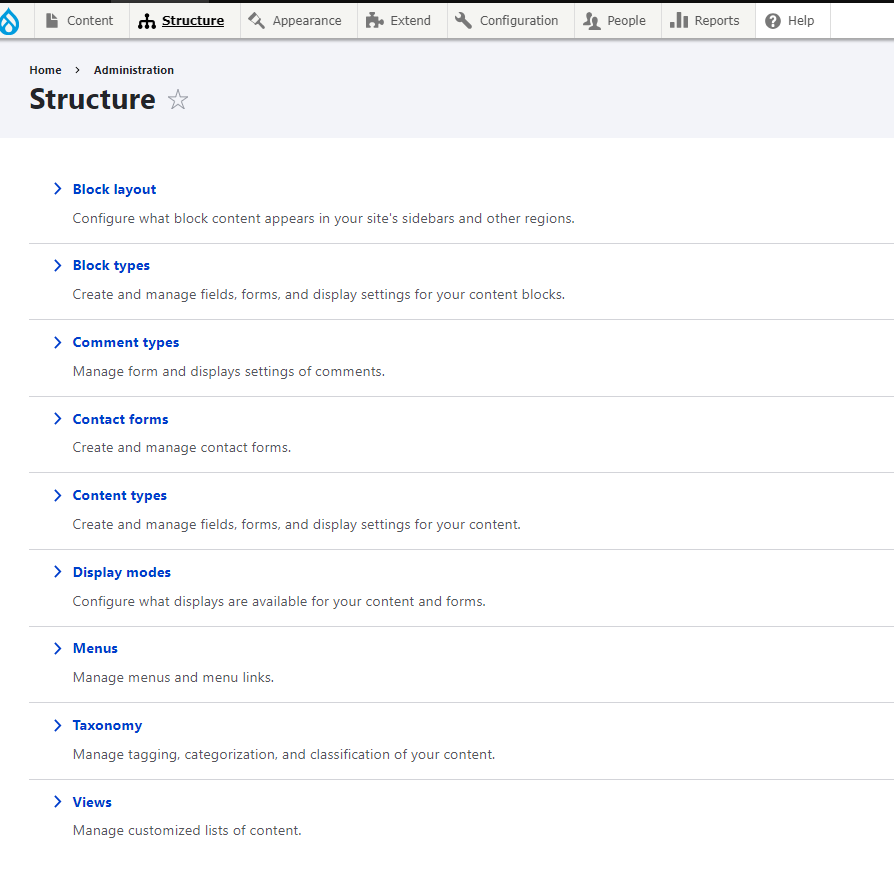
\includegraphics[width=1\linewidth]{img/ch4/admin_structure}
    \caption{Structural Elements}
    \label{fig:struct_elements}
\end{figure}

Each of these elements has a certain use within Drupal. The following list describes each of the structural elements. Don’t worry if not all the elements are clear to you, when you start changing and using your site the structure will become clear.
\\

\textbf{Block layout}: Blocks are site elements which can be positioned in different places on your site. For example, the search field, which is visible on the left side of your first Drupal page, is a Drupal block. You can put a block in different places on your page, these places are called \textbf{regions}. These regions depend on the Drupal theme you are using. When you click the \textbf{Block layout} link you will see the following page (Figure \ref{fig:admin_block_layout}).

\begin{figure}[H]
    \centering
    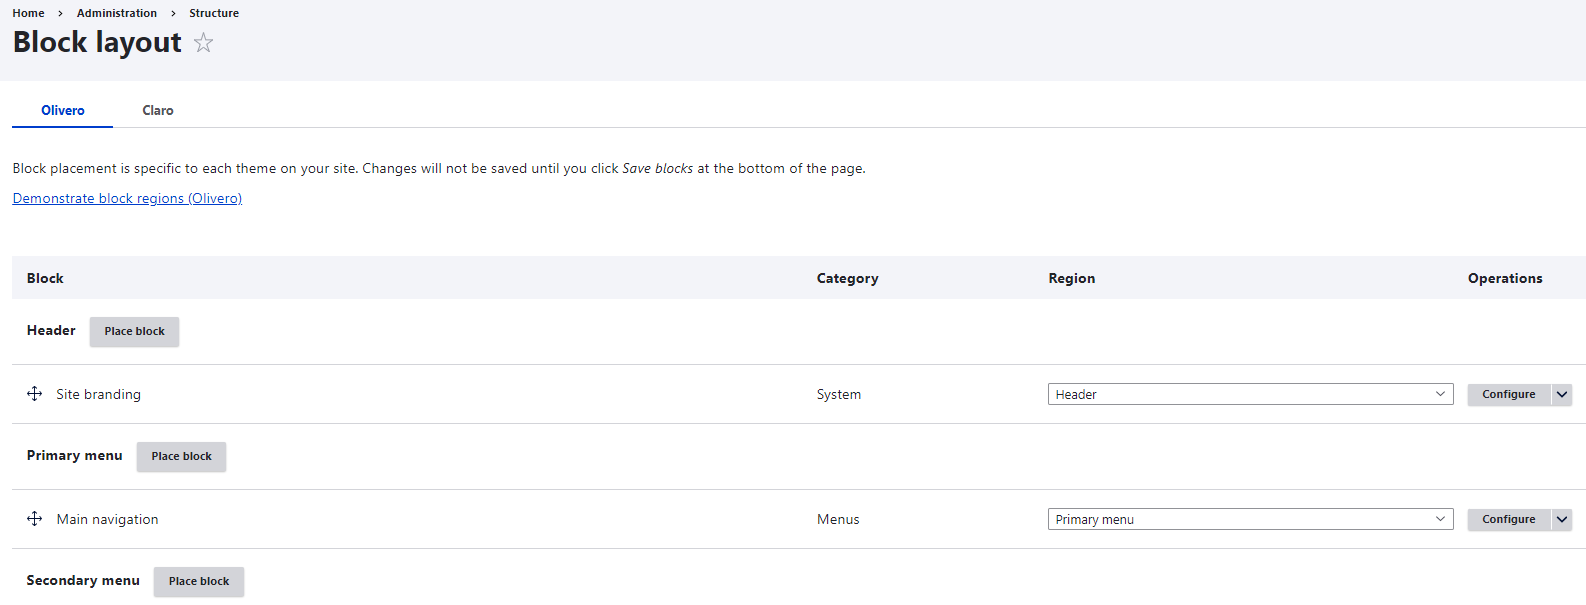
\includegraphics[width=1\linewidth]{img/ch4/admin_block_layout}
    \caption{Block Layout}
    \label{fig:admin_block_layout}
\end{figure}

\\
This page shows a list of the different regions and allows you to add blocks to each of these regions. You can click the link Demonstrate block regions(Olivero) to view the regions of the current theme (Olivero) (Figure \ref{fig:admin_region_demo}).

\begin{figure}[H]
    \centering
    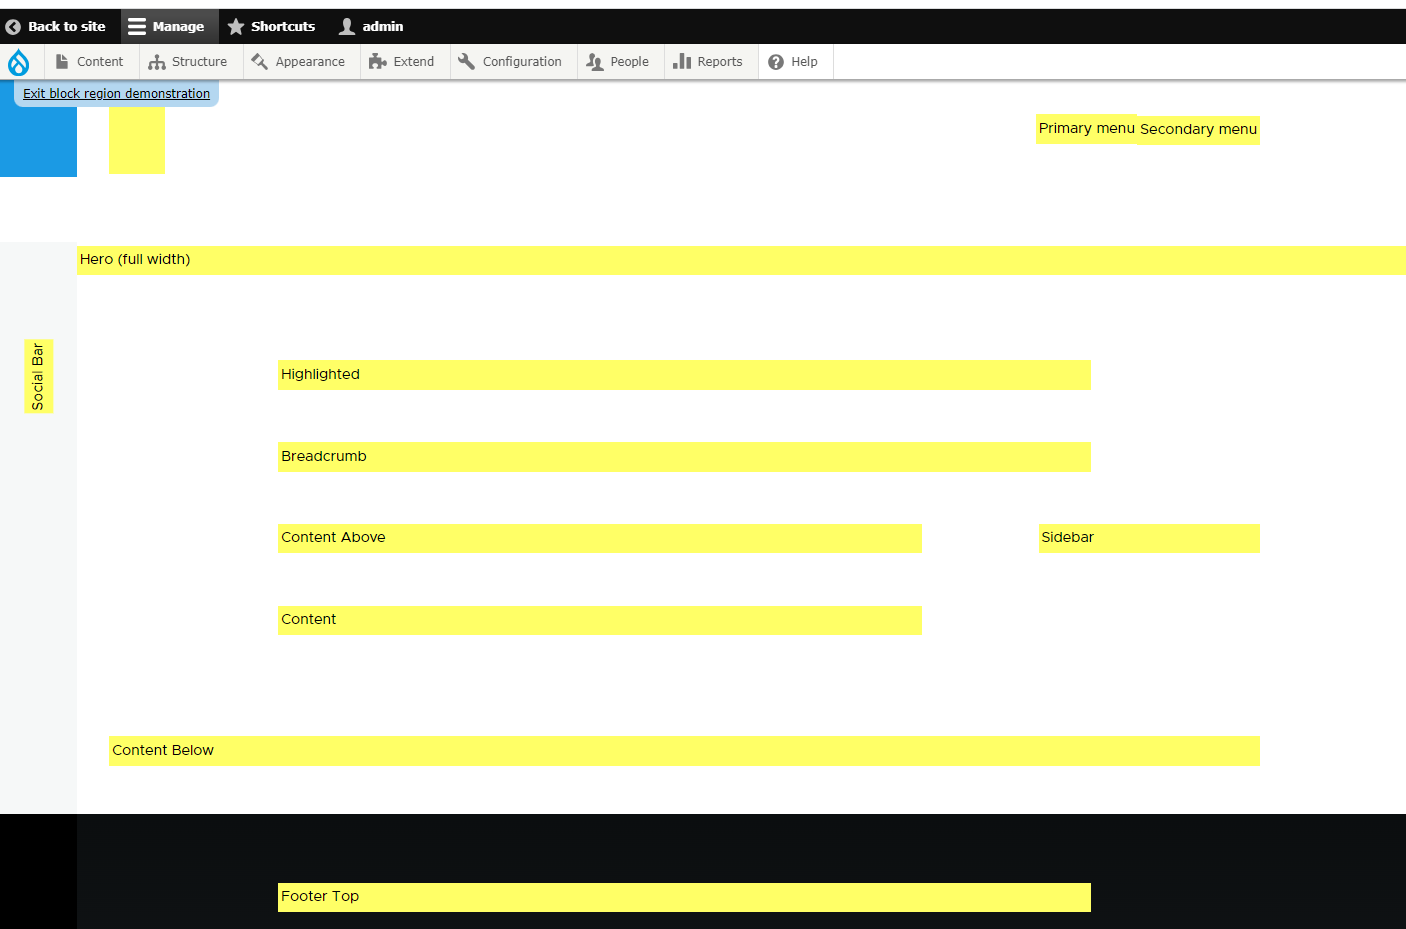
\includegraphics[width=1\linewidth]{img/ch4/admin_region_demo}
    \caption{Olivero regions}
    \label{fig:admin_region_demo}
\end{figure}

\\
\textbf{Comment types}: The comment types page allows you to create and manage different comment types. When you add content to your site you can allow people to comment on the new content. The comment type defines the fields that the commenter has to fill out when he’s writing his comment. The default comment type has only one field: the comment body. We could, for example, create a new comment type which includes a field for the name and age of the commenter.
\\
\textbf{Contact form}: The Personal contact form is the form for site visitors to contact registered users; the name and recipients of this form cannot be edited. Other forms listed here are your configured site-wide contact forms, which site visitors can use to send mail to a centralized email address or addresses. You can edit the name and recipients of site-wide forms by choosing the Edit operation. You can also configure the fields and display of both personal and site-wide forms.
\\
\textbf{Content types}: The content types page is very important. The content types define which kind of information your CMS will manage. A content type has different fields. These fields define the information that is stored in the content type. By default, Drupal has two content types: Article and Basic page (Figure \ref{fig:admin_content_types}).

\begin{figure}[H]
    \centering
    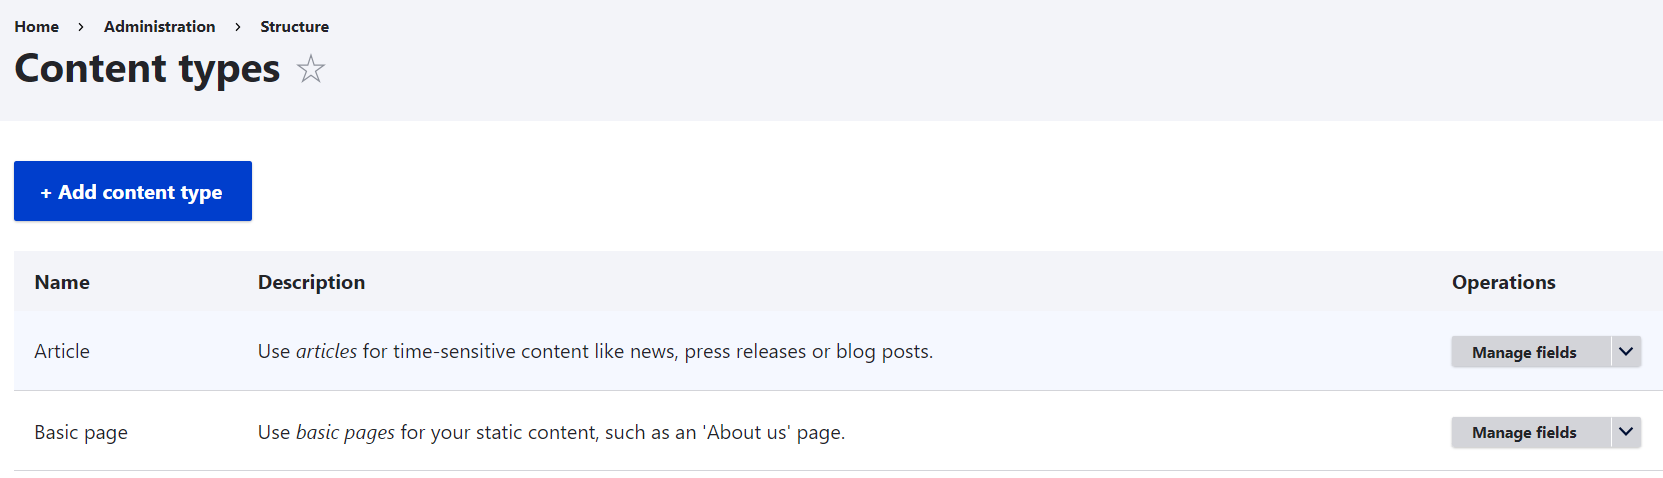
\includegraphics[width=1\linewidth]{img/ch4/admin_content_types}
    \caption{Default content types}
    \label{fig:admin_content_types}
\end{figure}


When you click the Manage fields button on the right you can see what kind of information is stored in this content type. (Figure \ref{fig:content_article_fields}). As you can see, the Article content type has four fields: Body, Comments, Image and Tags.

\begin{figure}[H]
    \centering
    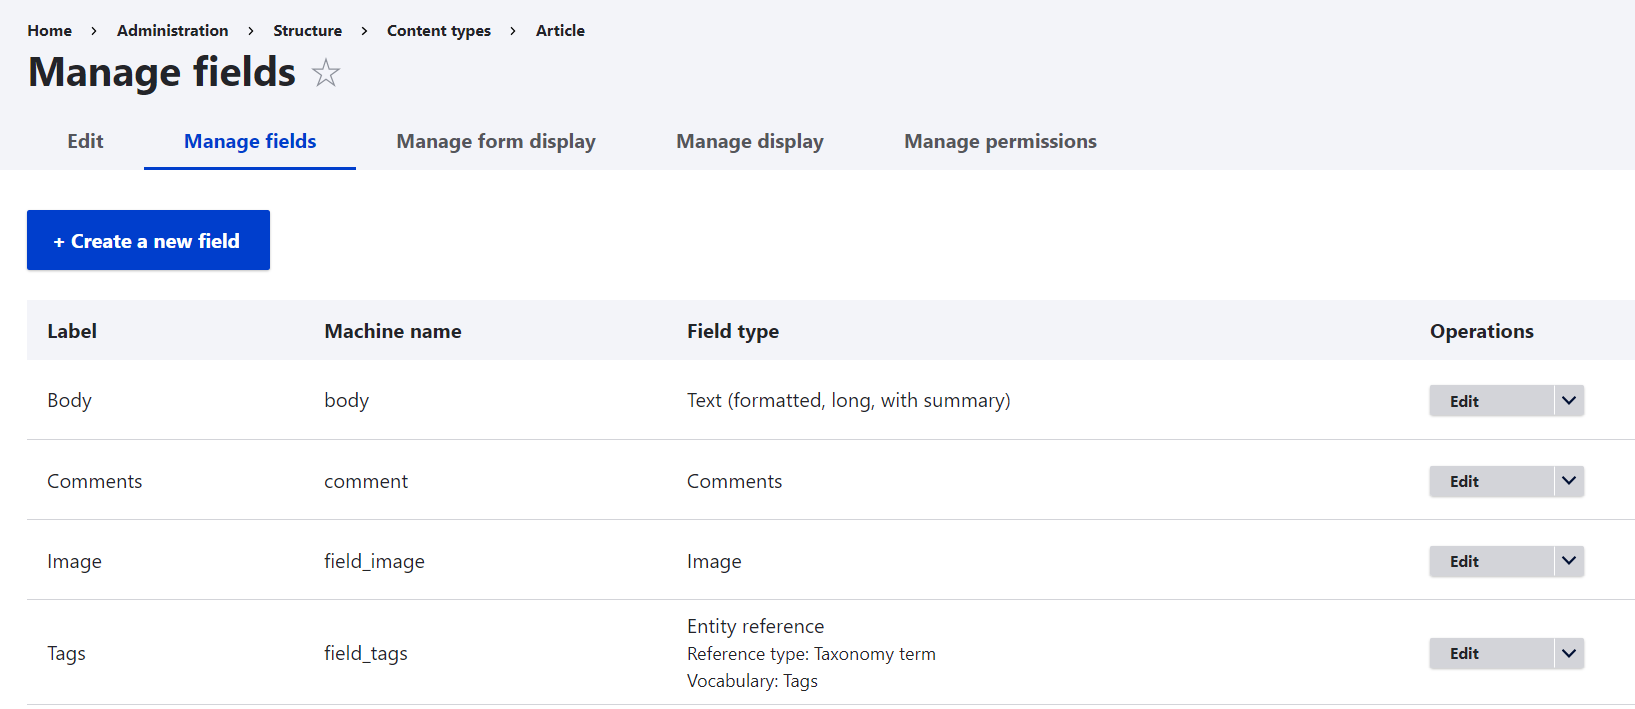
\includegraphics[width=1\linewidth]{img/ch4/content_article_fields}
    \caption{Article content type fields}
    \label{fig:content_article_fields}
\end{figure}

Next to the Manage fields menu item tab you have the Manage form display and Manage display tabs. These allow you to edit which fields are displayed when an element is created/edited or viewed.
\\
\textbf{Display modes}: Display modes define different ways in which information is displayed. There are two types of display modes: form modes and view modes. Form modes are used when the content is created or edited, view modes when the content is viewed. When you go to Display modes → View modes (Figure \ref{fig:structure_view_modes}) you will see the different ways in which a content type can be displayed.

\begin{figure}[H]
    \centering
    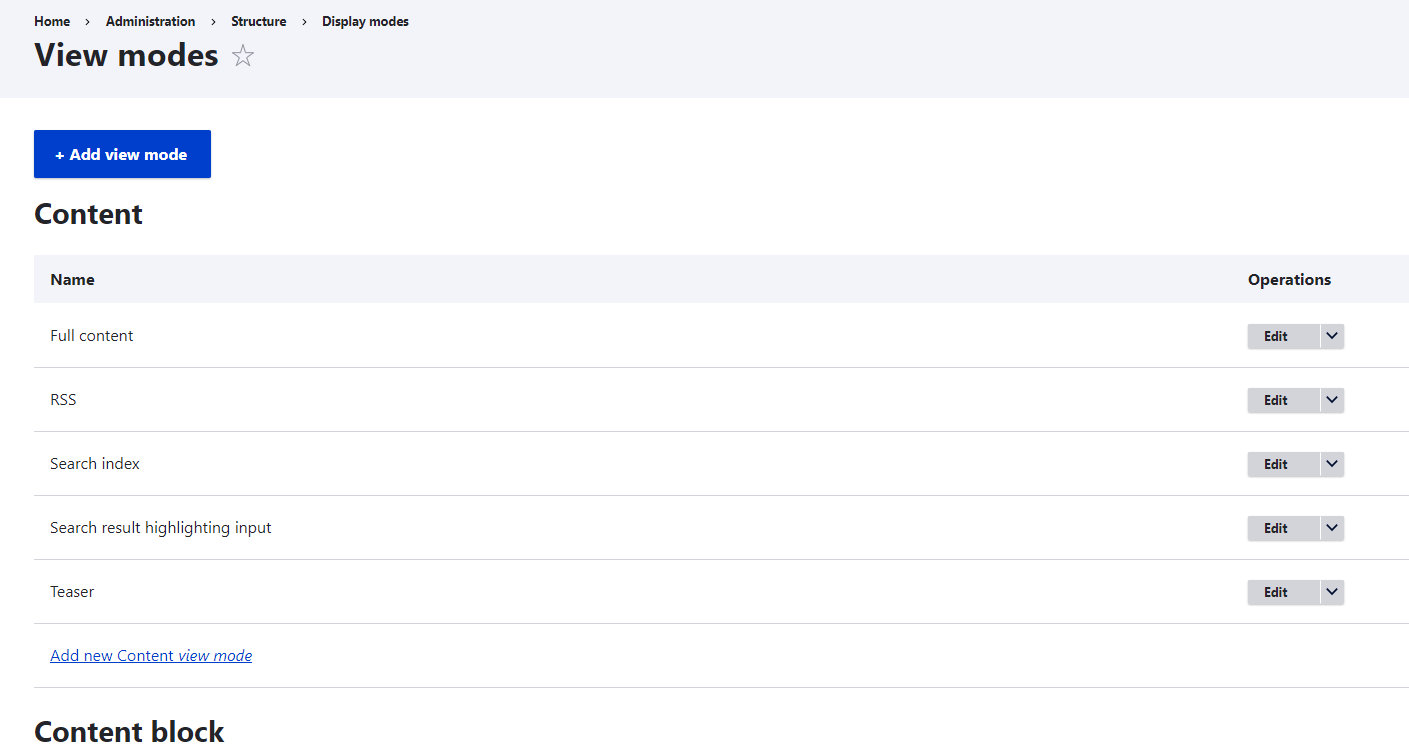
\includegraphics[width=1\linewidth]{img/ch4/structure_view_modes}
    \caption{Default view modes}
    \label{fig:structure_view_modes}
\end{figure}

When you go to Structure → Content types → Article → Manage display you will see the available display modes listed on top (Figure \ref{fig:article_display_mode}).

\begin{figure}[H]
    \centering
    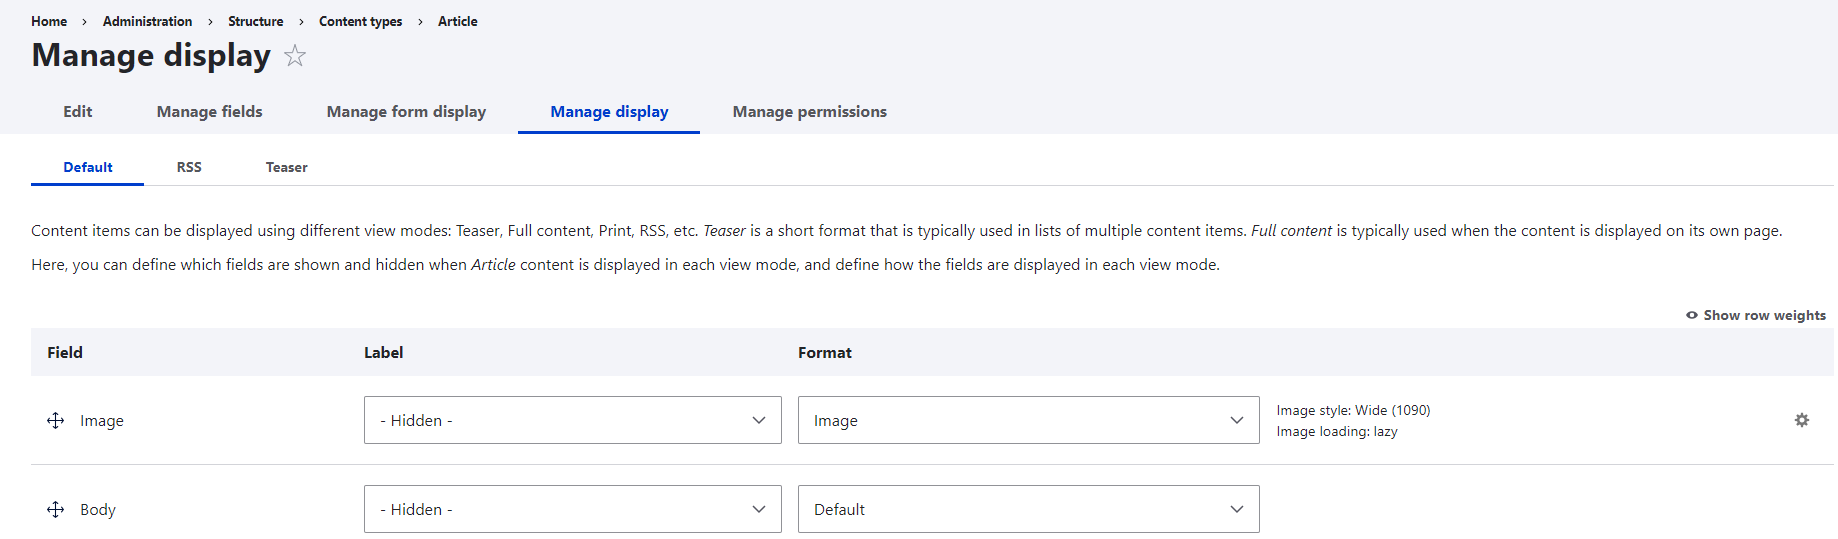
\includegraphics[width=1\linewidth]{img/ch4/article_display_mode}
    \caption{Article display modes}
    \label{fig:article_display_mode}
\end{figure}

There you see the different display modes that you can use for your Article content type. At the bottom of the page you can enable other display modes in the custom display settings dropdown (Figure \ref{fig:article_custom_display}).

\begin{figure}[H]
    \centering
    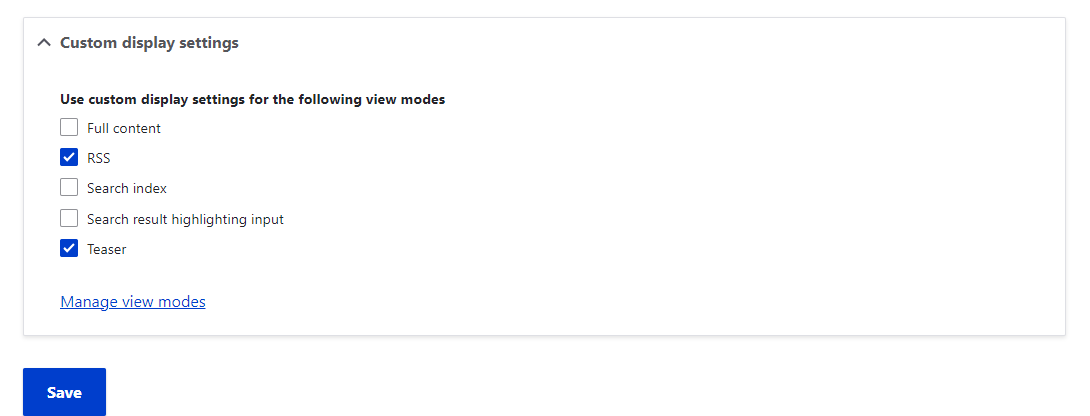
\includegraphics[width=1\linewidth]{img/ch4/article_custom_display}
    \caption{Custom display settings}
    \label{fig:article_custom_display}
\end{figure}

\\
\textbf{Menus}: Menus are easy. They define a menu with different menu items. Each menu has a corresponding block that is managed on the Block layout page.
\\
\textbf{Taxonomy}: A taxonomy defines lists of terms. These terms can be associated with the content. A list of terms is called a vocabulary. For example: if we have a site with news articles about sports we could add a tag to each article to tell what the article is about. These tags can be defined in a vocabulary.
\\
\textbf{Views}: A view enables you to create a display based on different content types. This course has a whole chapter dedicated to Drupal Views so we won’t go into details here.

\section{Our example}
\subsection{Change the site title and logo}
To make our site a little bit prettier we will change the logo and title. To change the site title, go to Configuration → System → Basic Site settings. Change the site name there to 'News First'  (Figure \ref{fig:admin_site_details}).

\begin{figure}[H]
    \centering
    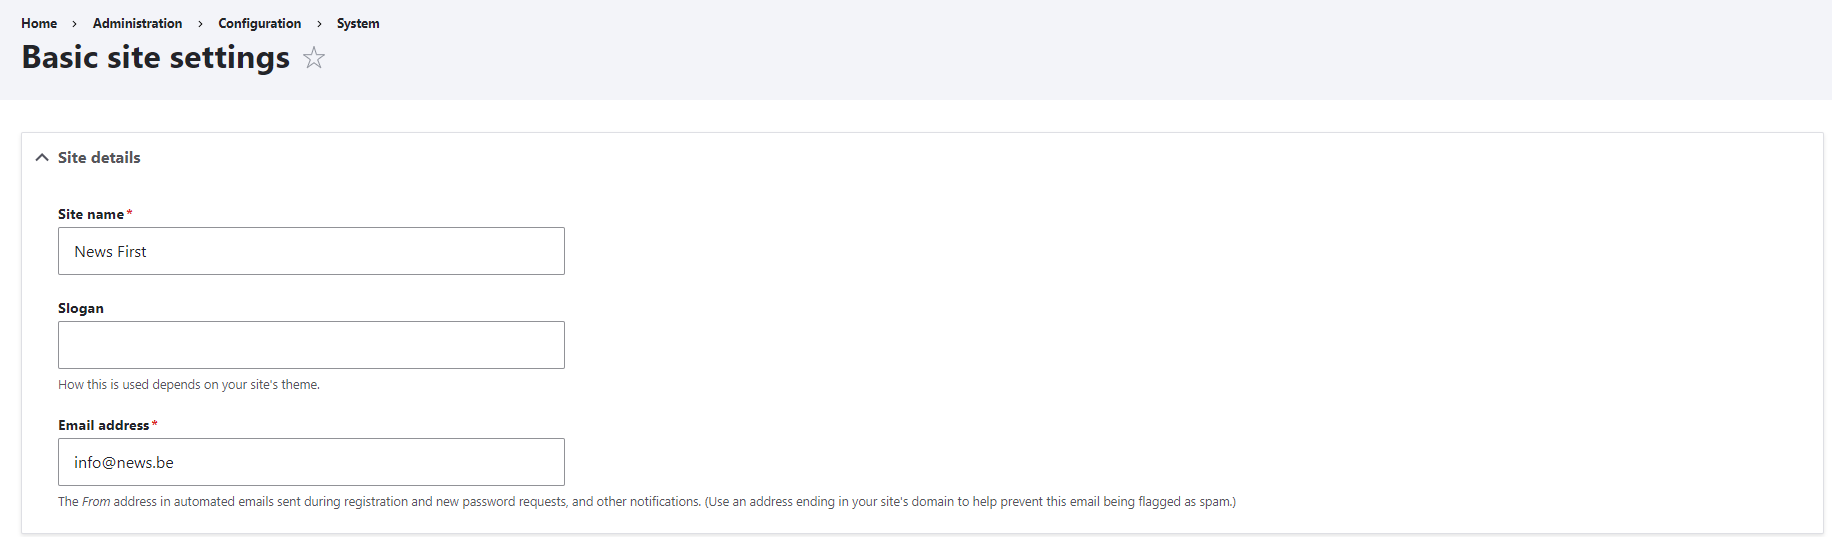
\includegraphics[width=1\linewidth]{img/ch4/admin_site_details}
    \caption{Changing the site title}
    \label{fig:admin_site_details}
\end{figure}

The logo is part of the Drupal theme you are using. To change the logo, go to: Appearance → Settings → Global Settings → LOGO IMAGE. Uncheck Use the default logo supplied by the theme and upload the file newssite\textunderscore logo.png (Available in the course files zip). Click Save configuration.

\begin{figure}[H]
    \centering
    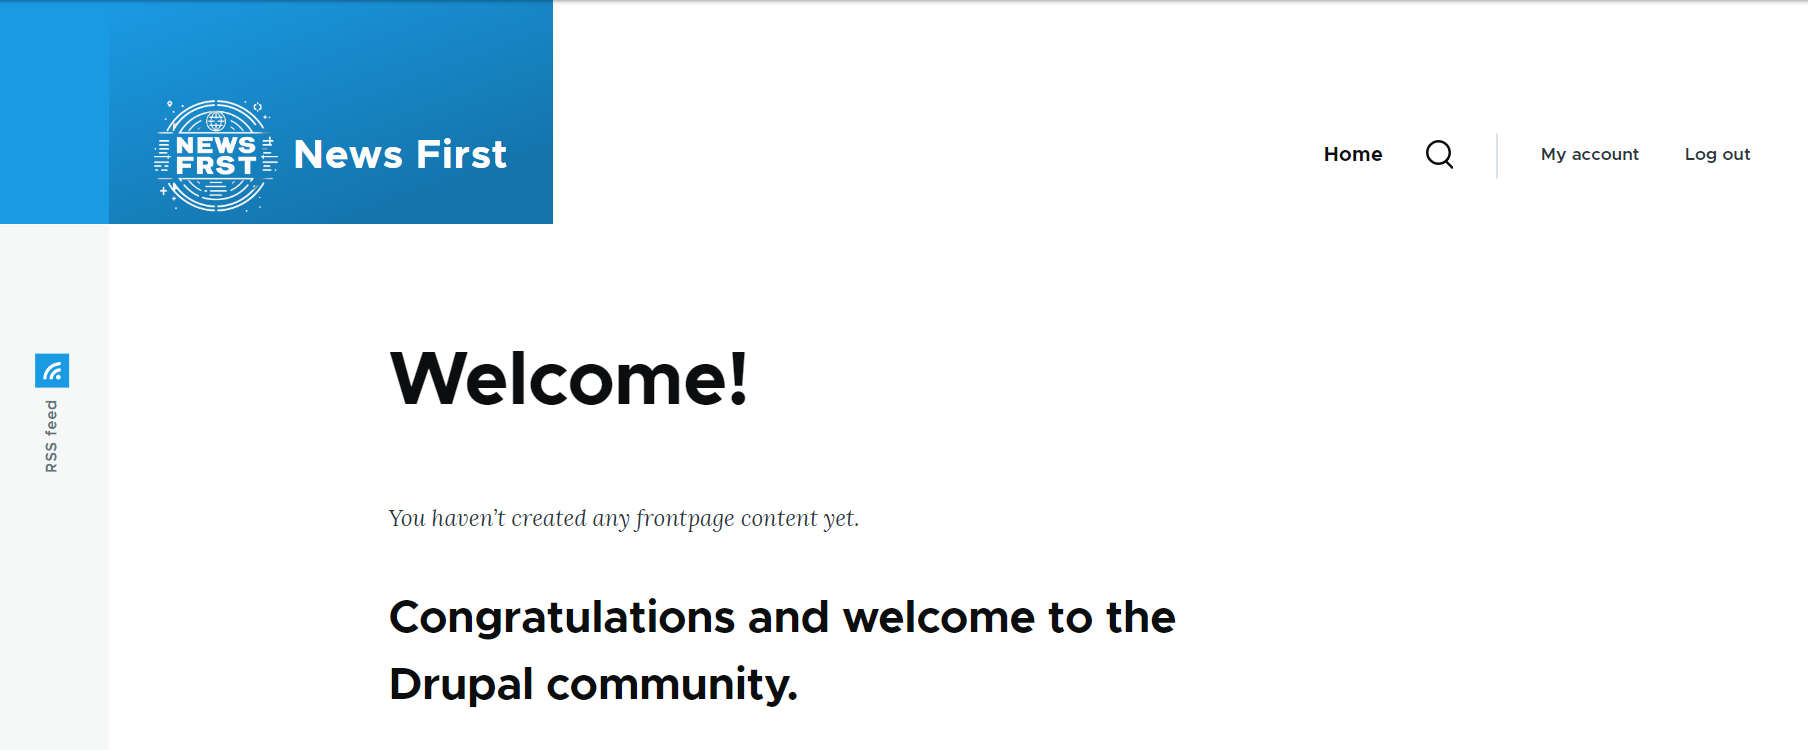
\includegraphics[width=1\linewidth]{img/ch4/site_main_logo}
    \caption{Changed logo and title}
    \label{fig:site_main_logo}
\end{figure}


\subsection{Removing unnecessary blocks}
Currently we don't need to have a search option nor the RSS feed. We can remove them by going to Structure → Block layout and disabling them. (Figure \ref{fig:admin_disable_block}). Click Save blocks to confirm the new layout.

\begin{figure}[H]
    \centering
    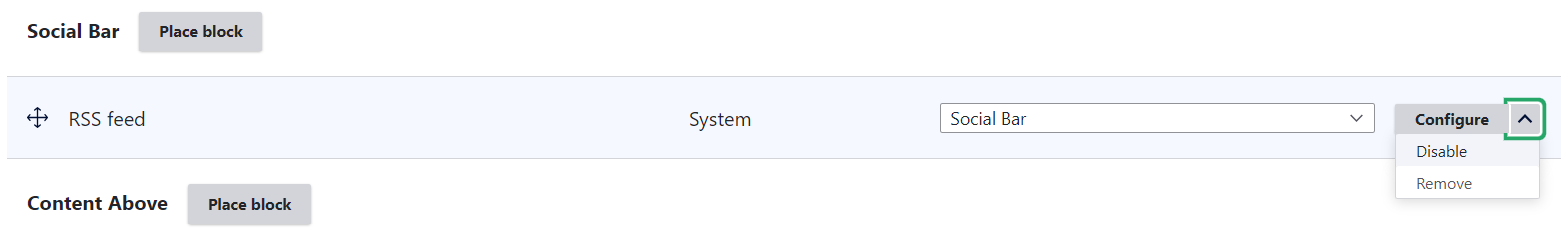
\includegraphics[width=1\linewidth]{img/ch4/admin_disable_block}
    \caption{Disabling an existing block }
    \label{fig:admin_disable_block}
\end{figure}

\subsection{Adding a Taxonomy}
To categorize the new items on our site we will add a taxonomy. This taxonomy will contain different types of news. Go to Structure → Taxonomy → Add vocabulary. Use the following settings:
\textbf{Name}: News Categories
\\
\textbf{Description}: Describes the type of the news item.
\\
Click Save. In Figure \ref{fig:admin_taxonomy_terms} you can see the empty vocabulary. Next we will add some terms to the vocabulary.

\begin{figure}[H]
    \centering
    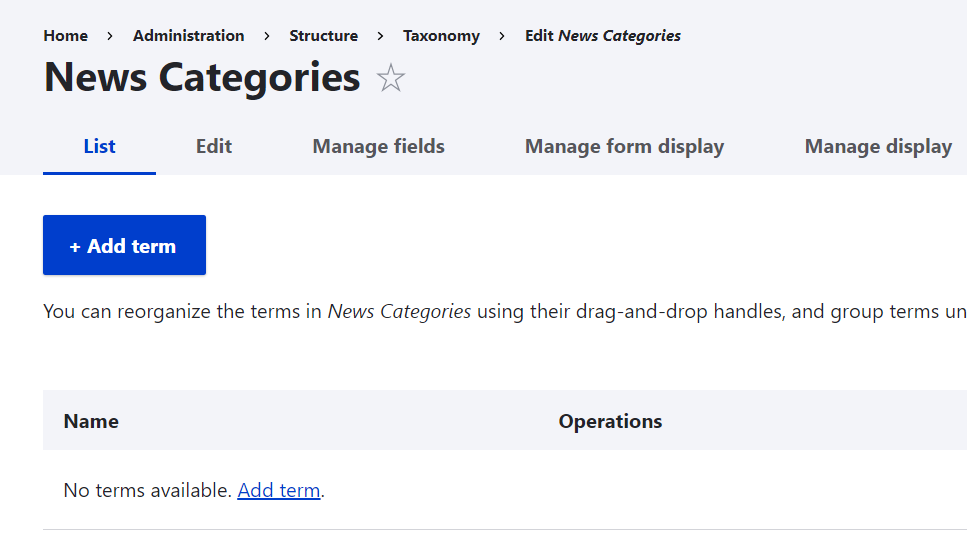
\includegraphics[width=1\linewidth]{img/ch4/admin_taxonomy_terms}
    \caption{Adding vocabulary terms }
    \label{fig:admin_taxonomy_terms}
\end{figure}

Click the Add term button and add the following terms:
\begin{itemize}
    \item national news
    \item international news
    \item sports 
    \item media
\end{itemize}

\begin{figure}[H]
    \centering
    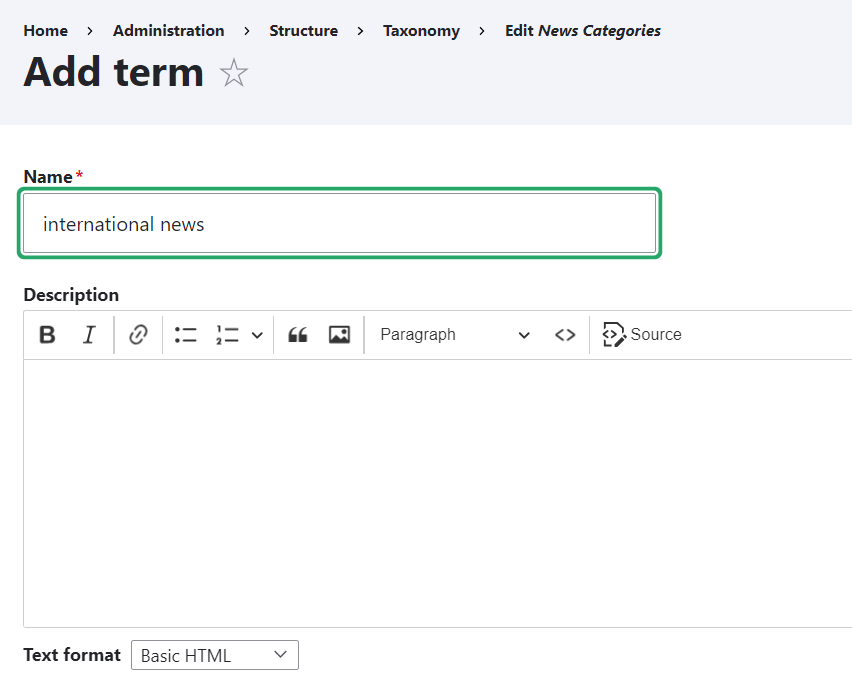
\includegraphics[width=1\linewidth]{img/ch4/admin_taxonomy_add}
    \caption{Adding vocabulary terms }
    \label{fig:admin_taxonomy_add}
\end{figure}

To see an overview of the terms you have added go to Structure → Taxonomy and click the List items button next to your vocabulary. (Figure \ref{fig:admin_taxonomy_list})


\begin{figure}[H]
    \centering
    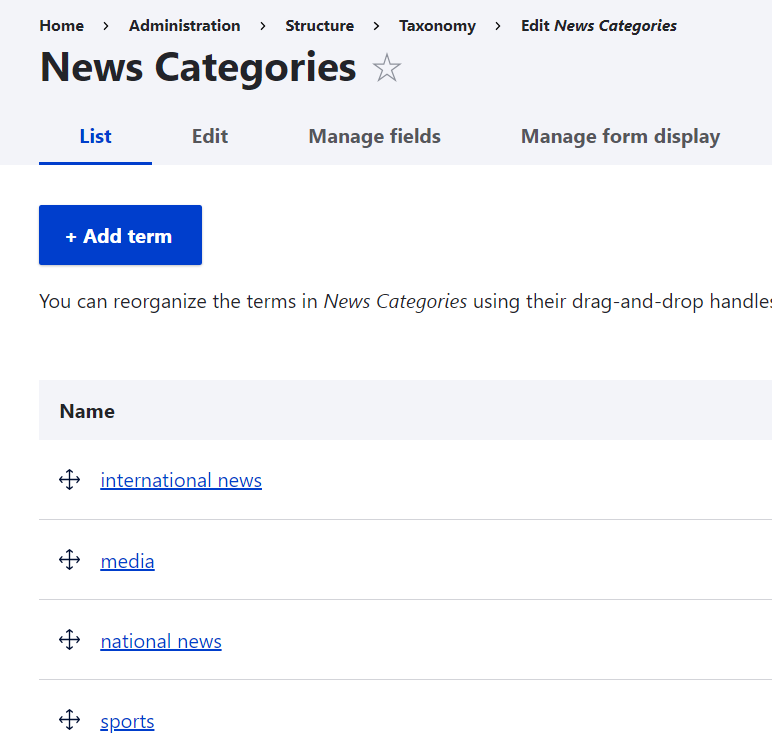
\includegraphics[width=1\linewidth]{img/ch4/admin_taxonomy_list}
    \caption{Vocabulary terms}
    \label{fig:admin_taxonomy_list}
\end{figure}


\subsection{Adding the News Item content type}
Since we are going to store news items in our CMS we will need to add the News Item content type. Go to: Structure → Content types → Add content type.
Give it the following properties:
\textbf{Name}: News Item
\\
\textbf{Description}: Some news!
\\
At the bottom of the page you can see some settings for this content type. Explore the settings, the names are very descriptive so most of them should be clear without further explanation. These are general settings that apply to all instances of this content type. You are able to change these for each instance individually when you create them. In most cases, when you create a new content type, you always want to untick the boxes under 'Menu settings'. It's highly unlikely that you want new content to be added to a menu. 
So go ahead and untick the box 'Main navigation' in the 'Menu settings'. 

(Figure \ref{fig:contenttype_news_add})


\begin{figure}[H]
    \centering
    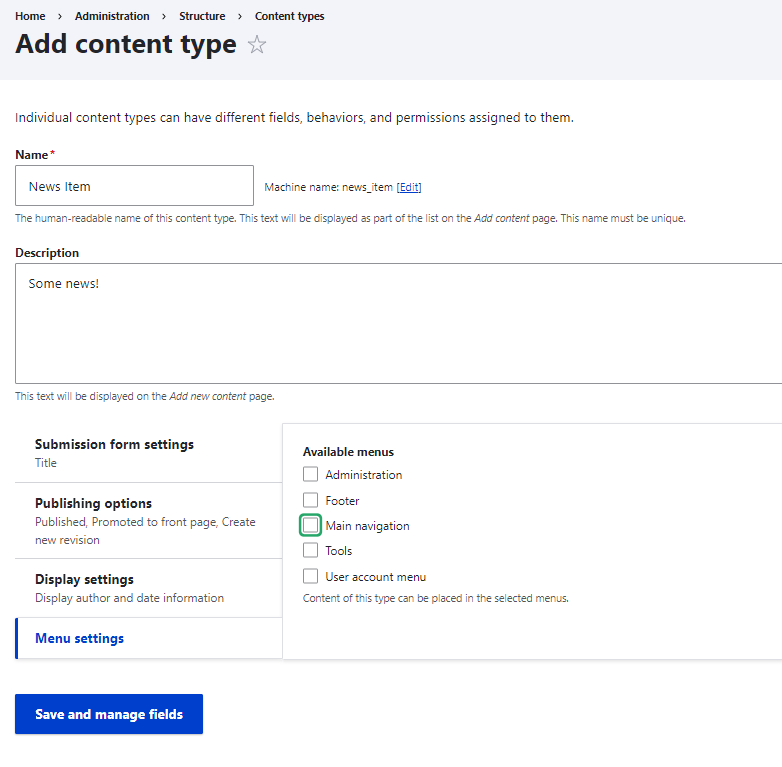
\includegraphics[width=1\linewidth]{img/ch4/contenttype_news_add}
    \caption{Adding the News Item Content Type}
    \label{fig:contenttype_news_add}
\end{figure}

Click 'Save and manage fields'.

Add the following fields to the News Item content type: 
\textbf{Body}: (this item is already there, leave it as it is)
\\
\textbf{NewsTitle}: (Text/plain, Maximum length = 255, number of values = 1) 
\\
\textbf{News Item Image}: (Image, number of values = 1)
\textbf{News category}: (Taxonomy term, number of values = unlimited, reference method = default, Vocabulary: news categories, Create referenced entities if they don’t already exist).
In figure 4.16 you can see an overview of the fields.

Figure 4.16: News item fields
\section{Review exercises}
In the following exercises we will review the content of this chapter by applying it to an example website. In the previous chapter we created the bitingbugs example website through the Acquia Dev Desktop. In this and the following chapters we will keep adding features to this site. Our goal is to create a web store for selling edible insects. The site will also provide a database with recipes so people know how to cook with the insects.

\begin{enumerate}
    \item Log in to your bitingbugs site (created in the previous chapter). Change the site name to Biting Bugs, and upload the file \\ bitingbugs\textunderscore \textunderscore logo \textunderscore transp \textunderscore white\textunderscore right\textunderscore small.png (Available in the course files zip) as logo for the site, and bitingbugs-favicon.png as favicon.
    \item Disable the powered by Drupal block and the rss feed.
    \item Add a comment type Answer to your bitingbugs site. We will use the comment type to allow users to answer a question. The comment type has two fields: answer (a number between 0 and 100000) and motivation (a textual explanation describing how they got the answer).
    \item\ Add vocabulary Food types type recipe to your bitingbugs site. Add the following terms to the vocabulary: Indian, Chinese, vegetarian, vegan, baking, snack
    \item Add a new content type recipe to your bitingbugs site. The new content type has the following fields: Name (=Title), Ingredients (formatted, long), Directions (formatted, long, with summary), Plate image, Estimated time (integer, in minutes), Type (food types)
    Make sure the teaser only displays the Title and Image fields.
\end{enumerate}
